\documentclass[11pt,a4paper,twoside]{article}
\usepackage[margin=1in, headheight=14pt]{geometry}
\usepackage{amsfonts,amsmath,amssymb,suetterl}
\usepackage{lmodern}
\usepackage[T1]{fontenc}
\usepackage{fancyhdr}
\usepackage{float}
\usepackage[utf8]{inputenc}
\usepackage{fontawesome}
\usepackage{enumerate}
\usepackage{xcolor}
\usepackage{hyperref}
\usepackage{tikz}
\usepackage{physics}
\usetikzlibrary{patterns, arrows.meta}

\DeclareUnicodeCharacter{2212}{-}

\usepackage{mathrsfs}
\usepackage[nodisplayskipstretch]{setspace}

\setstretch{1.5}
\renewcommand{\footrulewidth}{0pt}

\parindent 0ex
\setlength{\parskip}{1em}
\raggedbottom

\begin{document}
	\begin{singlespace}
		\begin{center}
			\Huge Queen Mary\\
			\LARGE University of London
		\end{center}
		\Large \textbf{MTH5123} \hfill \Large \textbf{Differential Equations,} \hfill \Large \textbf{Autumn 2020}\\
		\large \textbf{Coursework 5: Week 11 - Solutions} \hfill \large \textbf{W. Huang}
		\rule{\textwidth}{0.4pt}
	\end{singlespace}
	%
	\textbf{I. Practice Problems}\par
	\textbf{A.} Find all fixed points of the system $\dot{y_1} = f_1(y_1,\ y_2)\ \dot{y_2} = f_2(y_1,\ y_2)$ with
	$$
	f_1(y_1, y_2) = 2y_1 + y_2^2 - 1,\ f_2(y_1, y_2) = 6y_1 - y_2^2 + 1.
	$$
	Investigate the linear stability of the corresponding system linearized around each fixed point. Describe the type of fixed point and explain in words the shape of the trajectories close to it.\par
	\textbf{Solution:} To find all fixed points we solve the system
	$$
	f_1(y_1, y_2) = 0,\ f_2(y_1, y_2) = 0.
	$$
	From the first equation we obtain $y_1 = (1 - y_2)^2/2$. Substituting this into the second equation gives
	$$
	6y_1 - y_2^2 + 1 = 3(1 - y_2^2) - y_2^2 + 1 = 4(1 - y_2^2) = 0,
	$$
	which yields $y = \pm 1$ and $x = 0$. Therefore there exists two fixed points in the $(y_1, y_2)$ plane $0, 1$ and $0, -1$. Linearization around any equilibrium $(x^*, y^*)$ is based on the matrix
	$$
	A =
	\begin{pmatrix}
		\frac{\partial f_1}{\partial y_1}|_{y_1 = y^*, y_2 = y_2^*} & \frac{\partial f_1}{\partial y_2}|_{y_1 = y^*, y_2 = y_2^*}\\
		\frac{\partial f_2}{\partial y_1}|_{y_1 = y^*, y_2 = y_2^*} & \frac{\partial f_2}{\partial y_2}|_{y_1 = y^*, y_2 = y_2^*}
	\end{pmatrix}
	=
	\begin{pmatrix}
		2 & 2y_2^*\\
		6 & -2y_2^*
	\end{pmatrix}.
	$$
	For the first fixed point $(0, 1)$, we have $y_1^* = 0,\ y_2^* = 1$ yielding 
	$
	A =
	\begin{pmatrix}
		2 & 2\\
		6 & -2
	\end{pmatrix}
	$.
	The characteristic equation is given by $(2-\lambda)(-2-\lambda) - 12 = \lambda^2 - 16 = 0$. The eigenvalues are real and of different sign, $\lambda_1 = 4$ ann $\lambda_2 = -4$ showing that the equilibrium is a saddle, and trajectories close to it are hyperbolas. Using the corresponding eigenvectors $\vb{u_1} = \begin{pmatrix}1 \\ 1\end{pmatrix}$ and $\vb{u_2} = \begin{pmatrix}1 \\ -3\end{pmatrix}$,  you can plot the invariant manifolds and the phase portrait in the original coordinates as in Figure 1.
	%
	\begin{figure}[H]
		\centering
		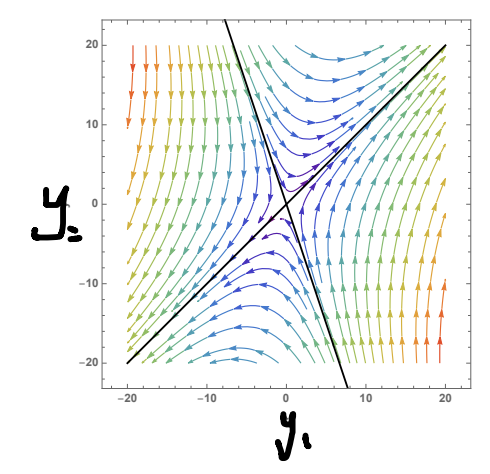
\includegraphics[width=0.5\textwidth]{figure/pdf27f1.PNG}
		\caption{ The phase portrait for problem A featuring a saddle at the equilibrium (0, 1). Note we plot the phase portrait by setting up the original at the equilibrium point.}
	\end{figure}
	%
	For the second fixed point $(0, -1)$, we have $y_1^* = 0,\ y_2^* = -1$ yielding
	$
	\begin{pmatrix}
		2 & -2\\
		6 & 2
	\end{pmatrix}
	$.
	The characteristic equation is given by $(2 - \lambda)^2 - 12 = \lambda^2 - 4\lambda + 16 = 0$. The eigenvalues are complex conjugate with positive real part, $\lambda = 2\pm i\sqrt{12}$ showing that the equilibrium is an unstable focus, and trajectories close to it are spiralling away from it. Note there are no invariant manifolds because the eigenvalues are complex numbers, and the corresponding phase portrait in the original coordinates are sketched in Figure 2.
	%
	\begin{figure}[H]
		\centering
		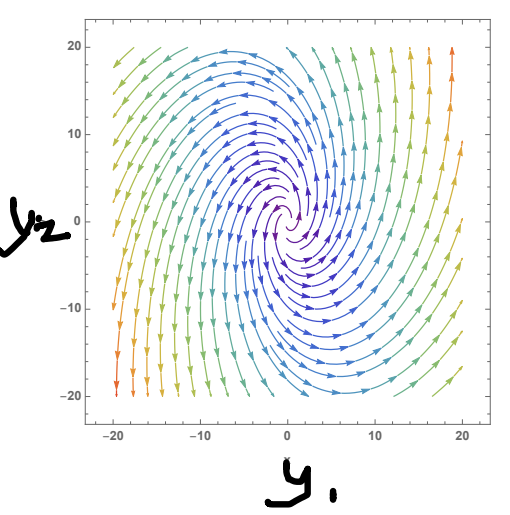
\includegraphics[width=0.5\textwidth]{figure/pdf27f2.PNG}
		\caption{The phase portrait for problem A featuring an unstable focus at the equilibrium $(0, -1)$. Note we plot the phase portrait by setting up the original at the equilibrium point}
	\end{figure}
	%
	\textbf{B.} Find the values of the real parameter a for which the system
	$$
	\dot{y_1} = y_2 + ay_1 - y_1^5,\ \dot{y_2} = -y_1 - y_2^5
	$$
	has a stable fixed point at $y_1 = y_2 = 0$. Use the function $V(y_1, y_2) = y_1^2 + y_2^2$ for judging the stability of the nonlinear system when linear stability is insufficient.\par
	\textbf{Solution:} The linearized system takes the form $\dot{y_1} = y_2 + ay_1,\ \dot{y_2} = -y_1$. The corresponding matrix is given by
	$
	A = 
	\begin{pmatrix}
		a & 1\\
		-1 & 0
	\end{pmatrix}
	$,
	and the characteristic equation is $(a - \lambda)(-\lambda) + 1 = \lambda^2 - a\lambda + 1 = 0$ with the two roots
	$$
	\lambda_1 = \frac{a + \sqrt{a^2 - 4}}{2},\ \lambda_2 = \frac{a - \sqrt{a^2 - 4}}{2}.
	$$
	We need to consider three different cases:\\
	(\textbf{i}) $a^2 < 4$ or equivalently $-2 a < 2$: The two roots are complex conjugate,
	$$
	\lambda_1 = \frac{a + i\sqrt{4 - a^2}}{2},\ \lambda_2 = \frac{a - i\sqrt{4 - a^2}}{2}.
	$$
	We have $Re\lambda = \frac{a}{2}$, which is negative for $-2 < a < 0$ when the corresponding system is asymptotically stable and positive for $0 < a < 2$ when the system is unstable. For $a = 0$ the real part vanishes so that the fixed point is a center, hence stable linearly. But according to our theorem we cannot judge by linear analysis about the properties of the nonlinear system. Using the suggested function $V(y_1, y_2)$ in the case of $a = 0$ we obtain for its orbital derivative
	$$
	\mathcal{D}_fV = \frac{\partial V}{\partial y_1}\dot{y_1} + \frac{\partial V}{\partial y_2}\dot{y_2} = 2y_1(y_2 - y_1^5) + 2y(-y_1 - y_2^5) = -2y_1^6 - 2y_2^6 < 0\ \forall(y_1, y_2) \neq (0,0).
	$$
	According to the Lyapunov stability theorem we can thus conclude that the system is also (asymptotically) stable for $a = 0$.\\
	(\textbf{ii}) $a \geq 2$: The two roots are real and $\lambda_1 = \frac{a + \sqrt{a^2 - 4}}{2} > 0$, so the system is unstable.\\
	(\textbf{iii}) $a \leq -2$: Here the two real roots are both negative,
	$$
	\lambda_1 = \frac{-|a| + \sqrt{|a|^2 - 4}}{2} <0,\ \lambda_2 = \frac{-|a| - \sqrt{|a|^2 - 4}}{2} < 0,
	$$
	and the linear system is asymptotically stable. Hence the zero solution for the nonlinear system is stable as well.\par
	\textbf{C.} Study the stability properties of the solution $y_1(t) = 0$ of the second order differential equation
	$$
	\ddot{y_1} + (a - 1)\dot{y_1} + (4 - a^2)y_1 = 0
	$$
	for the values $a = 1,\ a= 2$ and $a = -2$ of the real parameter $a$ by converting the ODE to a system of two first-order equations.\par
	\textbf{Solution:} Introducing $\dot{y_1} = y_2$ as the first equation we have $\dot{y_2} = \ddot{y_1}$. Then one can rewrite the second-order ODE as
	$$
	\ddot{y_1} = -(a - 1)\dot{y_1} - (4 - a^2)y_1\ \Rightarrow \ \dot{y_2} = -(a - 1)y_2 - (4 - a^2)y_1,
	$$
	which together with $\dot{y_1} = y_2$ yields a system of two first-order linear equations.\\
	We see that the corresponding matrix is given by
	$
	A =
	\begin{pmatrix}
		0 & 1\\
		-(4 - a^2) & -(a - 1)
	\end{pmatrix}
	$
	The characteristic equation is $(-\lambda)(-(a - 1) - \lambda) + 4 - a^2 = \lambda^2 + (a - 1)\lambda + 4 - a^2 = 0$ with the two roots
	$$
	\lambda_1 = \frac{1 - a + \sqrt{5a^2 - 2a - 15}}{2},\ \lambda_2 = \frac{1 - a - \sqrt{5a^2 - 2a - 15}}{2}.
	$$
	We now consider the three different cases above:
	(\textbf{i}) If $a = 1$  we have two complex conjugate roots $\lambda_1 = i\sqrt{3},\ \lambda_2 = -i\sqrt{3}$. As the real part is vanishing the linear system has a centre. Although the zero solution of the system is stable, it is not asymptotically stable.\\
	(\textbf{ii}) If $a = 2$ we have two real roots $\lambda_1 = 0,\ \lambda_2 = -1 < 0$, hence the zero solution is again stable but not asymptotically stable.\\
	(\textbf{iii}) If $a = -2$ we have two real roots $\lambda_1 = 0,\ \lambda_2 = 3 > 0$, hence the zero solution is unstable.\par
	\textbf{D.} Analyze the nature and stability of the critical point $(0, 0)$ as a function of the parameters $L,\ R$ and $C$ for the dynamical system arising from the equation
	$$
	L \frac{d^I}{dt^2} + R\frac{dI}{dt} + \frac{1}{C} = 0.
	$$
	\textbf{Solution.} In Coursework 5 week 10, we rewrite the equation above as a system of two first-order differential equations for $y_1 = I$ and $y_2 = dI/dt$ and show that $y_1 = 0,\ y_2 = 0$ is a critical point of the system. For the stability analysis, we find
	\begin{align*}
		R^2 > 4L/C \quad \Rightarrow \quad \text{node, asymptotically stable}\\
		R^2 < 4L/C \quad \Rightarrow \quad \text{spiral point, asymptotically stable}
	\end{align*}
	%
	\textit{Note: when $R^2 = 4L/C$, there are equal eigenvalues, not investigated in detail in our lectures. In this case, we call the critical point an improper node (which, in this case, is asymptotically stable).}
\end{document}